\pagebreak

\section*{Q3}
\begin{solution}
\hfill\break
Code is given in separate file. 
\begin{figure}[H]
    \centering
    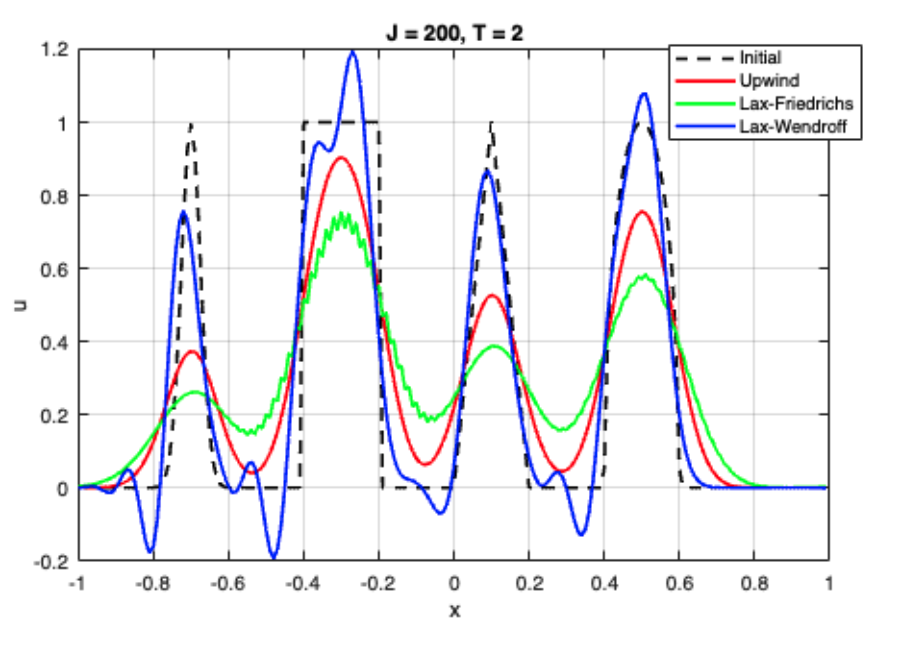
\includegraphics[scale=0.4]{./figures/q3-t2j200.png}
    \caption{Solution for $T = 2$ and $J = 200$.}
\end{figure}
\begin{figure}[H]
    \centering
    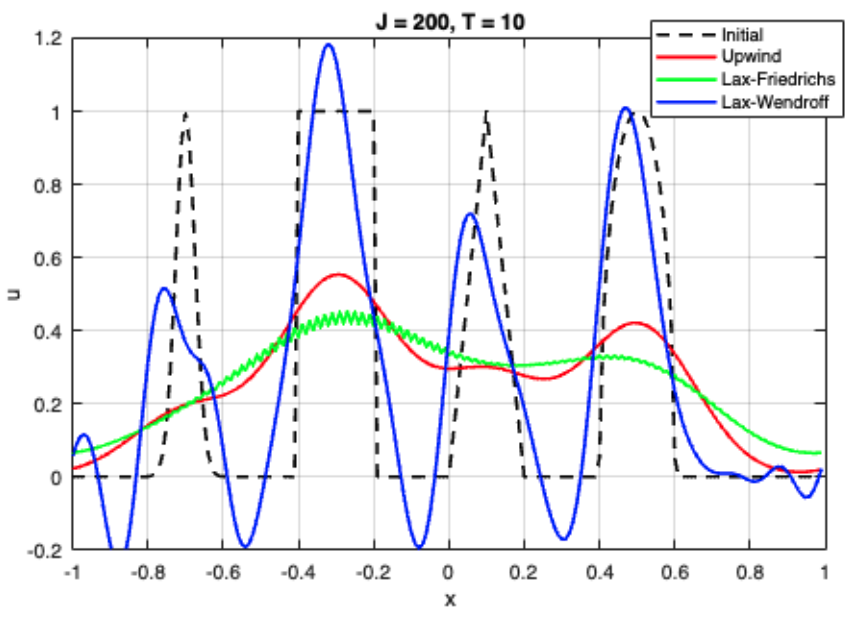
\includegraphics[scale=0.4]{./figures/q3-t10j200.png}
    \caption{Solution for $T = 10$ and $J = 200$.}
\end{figure}
\begin{figure}[H]
    \centering
    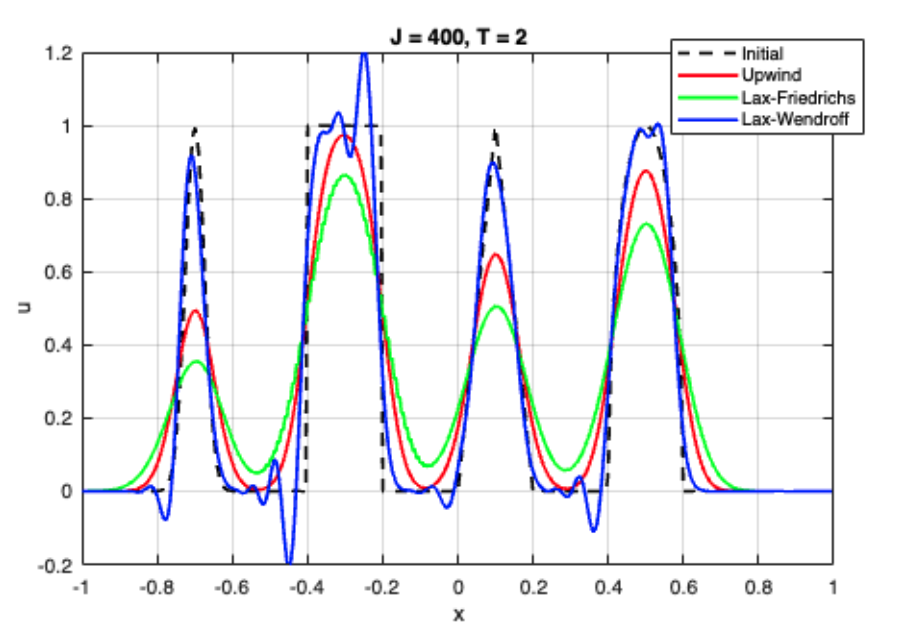
\includegraphics[scale=0.4]{./figures/q3-t2j400.png}
    \caption{Solution for $T = 2$ and $J = 400$.}
\end{figure}
\begin{figure}[H]
    \centering
    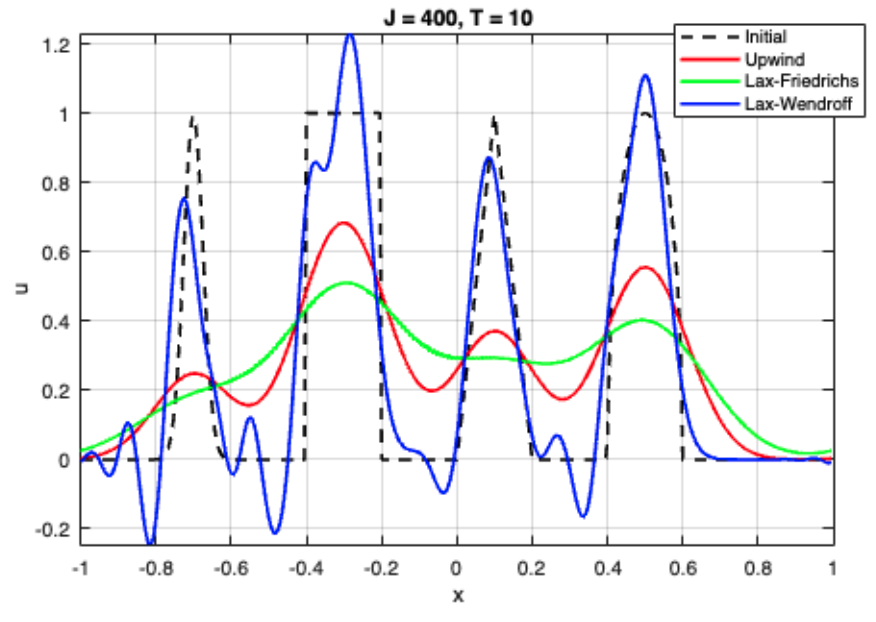
\includegraphics[scale=0.4]{./figures/q3-t10j400.png}
    \caption{Solution for $T = 10$ and $J = 400$.}
\end{figure}
We see here with a smaller $J$ value our curves are more jadded. For all cases, Lax-Friedrich particularly suffers from this shape where as Upwind and Lax-Wendroff are a better match. We see faster dissipation from the Lax-Friedrich method compared to the others. The Lax-Wendroff has the best matching to our $u$, Lax-Friedrichs has jagged and sharp oscilations. Upwind conssitently dissipates strongly at $T = 10$ and is mostly sinusoidal at $T = 2$. For all methods we see a drastic improvement by doubling $J$ from $200 \to 400$. We also see that Lax-Wendroff is the only method that can model the square region through small oscilations, where as the other methods struggle to fit a flat line.

\hfill\break
\hfill\break
Now, write a code for five-fold cross validation and use it to check whether adding sex in the model improves its predictive error.

Now, use standard bootstrap, residual bootstrap and wild bootstrap with $B = 1000$ to construct confidence intervals for the coefficients in the previous two models (the first using only body weight and the second using both body weight and sex). For wild bootstrap consider $v_i$ as Radamacher random variable, i.e. takes value $+1$ and $-1$, both with probabilities half.
\hfill\break
\hfill\break
Suppose we have two samples $\left\{ X_i \right\}_{i =1}^m$ and $\left\{ Y_j \right\}_{j = 1}^n$ drawn iid from the distributions $P$ and $Q$. We want to test for the equality of distributions, i.e.
\begin{align*}
H_0 : P = Q, H_1 : P \neq Q.
\end{align*}
As a possibility, lets consider the test (proposed by Baringhaus and Franz, 2004) which relies on the following inequality: if $X_1, X_2 \sim iid \ P$, and $Y_1, Y_2 \sim iid \ Q$ then,
\begin{align*}
T^* = \mathbf{E}\left[ \lVert X_1 - Y_1 \rVert_2 - \frac{1}{2} \lVert X_1 - X_2 \rVert_2 - \frac{1}{2} \lVert Y_1 - Y_2 \rVert_2 \right] \geq 0
\end{align*}
and the inequality becomes equality if and only if $P = Q$. Based on this, they construct a $U$-statistic-based test statsitic, described as below:
\begin{align*}
T_{m,n} = \frac{mn}{m + n} \left[ \frac{1}{mn} \sum_{i = 1}^{ m}\sum_{j = 1}^{ n } \lVert X_i - Y_j \rVert_2 - \frac{1}{2m^2} \sum_{i = 1}^{ m }\sum_{j = 1}^{ m } \lVert X_i - X_j \rVert_2 - \frac{1}{2n^2}\sum_{i = 1}^{ n} \sum_{j = 1}^{ n } \lVert Y_i - Y_j \rVert_2 \right]
\end{align*}
Notice the similarities between $T^*$ and $T_{m,n}$. Now, let's consider $m = n = 20$ and the following distributions,
\begin{align*}
X_i \sim iid \ \mathcal{N}(\mu_1, 1), Y_i \sim iid \ \mathcal{N}(\mu_2,1)
\end{align*}
Describe the rejection rule for a permutation test for the equality of distribution using the test statistic $T_{m,n}$ at a significance level $\alpha = 0.05$ and write a function for it in r. You can consider $B = 200$ as the number of random permutations.
\hfill\break
\hfill\break
Set $\mu_2 = 0$ and consider a sequence $\mu_1$ 's in a range of $[0,0.8]$ at an interval  0.1 (seq(0,0.8, by = 0.1) in r). For each $\mu$ generate $500$ samples and calculate the proportion of times the permutation test was rejected. These proportions of times are also known as the power of the test. Plot these proportions against $\mu$
\hfill\break
\hfill\break
Note that we didn't need to know anything about the distribution $P$ and $Q$. Such a test is called a non-parametric test. Now, lets compare this permutation test against an ideal test, where we do known that both the distributions are normals with variance one, but the means are unknown. So, testing $P = Q$ is equivalent to testing $\mu_1 = \mu_2$. In this case, the test statistic is,
\begin{align*}
T = \sqrt{\frac{mn}{m + n}} (\overline{X} - \overline{Y}),\ \overline{X} = \frac{1}{m}\sum_{i = 1}^{ m}X_i, \ \overline{Y} = \frac{1}{n} \sum_{i = 1}^{ n }Y_i
\end{align*}
and under $H_0: T \sim \mathcal{N}(0,1)$. Using this test statistic, construct a rejection rule for $\mu_1 = \mu_2$ against $\mu_1 \neq \mu_2$ at $\alpha = 0.05$ and in a similar setting as before calculate the proportions of time the test was rejected at different $\mu_1$. You should use the same samples that you generated as in the previous example. Compare both power curves for the two tests in a plot.
\hfill\break
\hfill\break
When $\mu_1 = 0$, the two distributions are identical, so the rejection proportion should be around $0.05$, matching the false positive rate we set by $\alpha$. Both samples are drawn from $\mathcal{N}(0,1)$ meaning any statistical hypothesis test (in our case the permutation test) is controlled by the significance level $\alpha$. In our case $\alpha = 0.05$ meaning we will incorrectly reject the null hypothesis about $5\%$ of the time when the null is actually true. Therefore the rejection proportion when $\mu_1 = 0$ should be approximately $0.05$.
\hfill\break
\hfill\break
Given a test statistic $T_{m,n}$ and a significance level $\alpha = 0.05$, the rejection rule for a two-sample permutation test is based on p-value in the permutation test algorithm. First we randomly permute the combined sample $(X_1,\dots,X_m,Y_1,\dots,Y_n)$ and reassign $m$ and $n$ values and compute $t^{(b)}$ for each permutation $b = 1,\dots,B$. Then we compute the $p$-value,
\begin{align*}
p = \frac{1}{B} \sum_{b = 1}^{ B} \mathbb{I} \left\{ t^{(b)} \geq t_{\text{obs}} \right\}
\end{align*}
where $t^{b} = T(U_1^{(b)}, \dots, U_{m+n}^{(b)})$ and $t_{\text{obs}}$ is the calculated test statistic for the original unpermuted data. We reject rule is governed by checking if $p < \alpha = 0.05$, which means we reject the null hypothesis $H_0$.
\hfill\break
\hfill\break
Let's consider a 2-dimensional donut distribution whos density is proportional to,
\begin{align*}
p(x,y) \propto \exp \left( - \frac{x^2 + y^2}{2} - 8 ((x^2 + y^2)^{\frac{1}{2}} - 3)^2\right)
\end{align*}
Starting from the state $(2,0)$, implement random-walk Metropolis-Hastings in R to draw samples from this distribution. For the random-walk Metropolis-Hastings, consider standard deviations 0.1, 0.25, 0.5, and 1. Create a scatter plot for the first 100 samples drawn from the chains. Also, report the proportions of times the states were accepted within the first 2000 draws from each of the chains.
\hfill\break
\hfill\break
Do the same for Hamiltonian Monte Carlo. Try different step sizes (0.01, 0.05, 0.1) and number of steps (20,50) within the leapfrom approximation.
\hfill\break
\hfill\break
Consider the cats dataset in the library MASS. Let's consider a linear regression model to regress heart weight on body weight, ensuring that the regression line goes through the origin. 
\hfill\break
\hfill\break
We want to use a Bayesian approach to fit the linear regression model:
\begin{align*}
y_{i} = \beta x_{i} + \epsilon_i, \ \ \epsilon_i \sim \mathcal{N}(0,\sigma^2)
\end{align*}
Consider the conjugate priors $\beta \sim \mathcal{N}(0,\sigma^2)$ and $\sigma^2 \sim \text{Gamma}(1,1)$. Derive a Gibbs sampler for $\beta$ and $\sigma^2$.
\hfill\break
\hfill\break
Consider the cats dataset in the library MASS in r. Let's consider a linear regression model to regress heart weight on body weight, ensuring that the regression line goes through the origin. Use the Gibbs sampler to draw sample for $\beta$ from the posterior distribution. Using a histogram compare it to the maximum likelihood extimate of $\beta$ that you would obtained from the frequentist's approach to a linear regression model. Also, calculate a $95\%$ confidence interval for $\beta$ drawn from the Gibbs sampler and compare it to the frequentist's confidence interval.
\end{solution}
